 
\begin{center}
\resizebox{.5\textwidth}{.3\textheight}{
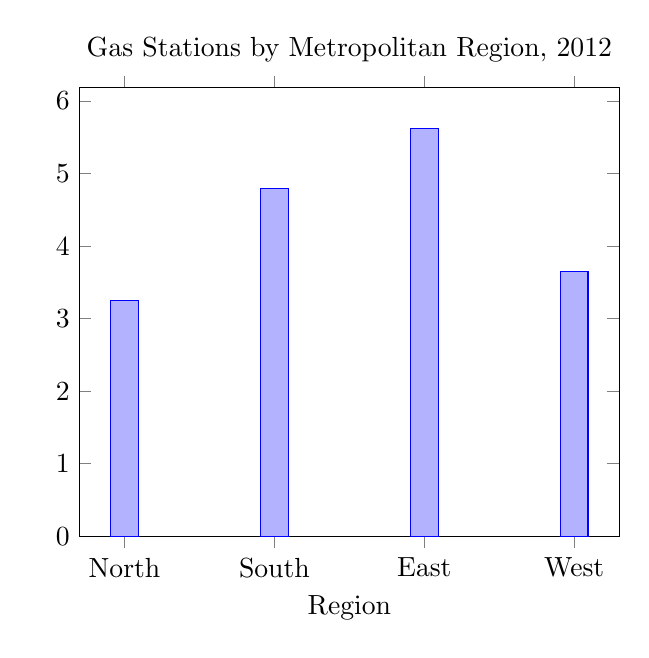
\begin{tikzpicture}
\begin{axis}[xtick={1,2,3,4},xticklabels={North, South, East, West}, ybar, ymin=0, ylabel=\empty, xlabel=Region, ytick={0,100,200,300,400,500,600}, yticklabels={0,1,2,3,4,5,6}, title={Gas Stations by Metropolitan Region, 2012}]
\addplot coordinates {(1,325)(2,480)(3,562)(4,365)};
\end{axis}\end{tikzpicture}}\end{center}

The number of gas stations in $4$ different regions of a metropolitan area is 2012 is shown in the graph above.  If the total number of gas stations is $1,732$, what is an appropriate label for the vertical axis of the graph?



\ifsat
	\begin{enumerate}[label=\Alph*)]
		\item  Number of gas stations 
		\item  Number of gas stations (in tens)
		\item  Number of gas stations (in hundreds) % 
		\item  Number of gas stations (in thousands)
	\end{enumerate}
\else
\fi

\ifacteven
	\begin{enumerate}[label=\textbf{\Alph*.},itemsep=\fill,align=left]
		\setcounter{enumii}{5}
		\item  Number of gas stations 
		\item  Number of gas stations (in tens)
		\item  Number of gas stations (in hundreds) % 
		\addtocounter{enumii}{1}
		\item  Number of gas stations (in thousands)
		\item None of these. 
	\end{enumerate}
\else
\fi

\ifactodd
	\begin{enumerate}[label=\textbf{\Alph*.},itemsep=\fill,align=left]
		\item  Number of gas stations 
		\item  Number of gas stations (in tens)
		\item  Number of gas stations (in hundreds) % 
		\item  Number of gas stations (in thousands)
		\item None of these. 
	\end{enumerate}
\else
\fi

\ifgridin
  Number of gas stations (in hundreds) % 
		
\else
\fi

